% ----------------------------------------------------
% Methodology
% ----------------------------------------------------

\chapter{Salinometer Evaluation and Testing}\label{ch:testing}

The \gls{pcb} boards were delivered and tested.
Some design errors were found which include using op-amps that were rated for 6V instead of 3V3, missing a connection between VDDA and VCC, and footprints errors with both the temperature sensor and depth sensor.
The temperature sensor footprint was unable to be corrected, but the depth sensor could be corrected by flipping the depth sensor.

Once the circuitry was working and coded, the salinometer was tested.
The testing was conducted in two phases.
One phase before the probe was cast into epoxy resin and the other after the probe was cast into epoxy resin (section numbers?).
A summary of these tests is shown in~\reftbl{tab:testing-summary} and each test is discussed in further detail in the following sections.

The equipment used to verify these tests were a bench multimeter model Keysight U3401A which had voltage accuracy to $0.02\%$ and resistance accuracy to $0.1\%$.
% \textit{insert picutres, adc config, dac step, r^2 values}.

%chktex-file 44
\begin{longtblr}[
    caption = {A summary of the evaluation and testing of the salinometer.},
    label = {tab:testing-summary}
    ]{
    colspec = {|C|C|C|C|}
    }
    \hline
    \textbf{Test} & \textbf{Description} & \textbf{Ideal Result} & \textbf{Measured Result} \\
    \hline
    DAC Voltage Range & The range of voltages that the DAC can output from $0V$ to $V_{DD} = 3.3V$ & $0-3.3V$ & \\
    \hline
    ADC Accuracy & The average accuracy of the ADC in measuring voltages from $DAC_{MIN}$ to $DAC_{MAX}$ & $100\%$ & \\
    \hline
    Calibration Resistance & The resistance of the calibration resistor $R_{CAL}$ & $5\Omega$ & \\
    \hline
    Calibration Resistance using ADC & The resistance of the calibration resistor $R_{CAL}$ as measured using the ADC & $5\Omega$ & \\
    \hline
    Resistance Measuring Accuracy & The salinometer's average accuracy in measuring specific resistances & $100\%$ & \\
    \hline
    Linear Conductivity Measurement Au & Whether the sample of salt water had linear conductivity throughout a range of voltages or not using the gold electrodes with no fringe shield & Non-linear &  \\
    \hline
    Linear Conductivity Measurement Shielded Au & Whether the sample of salt water had linear conductivity throughout a range of voltages or not using the gold electrodes with the fringe shield & Linear & \\
    \hline
    Linear Conductivity Measurement Ti & Whether the sample of salt water had linear conductivity throughout a range of voltages or not using the titanium electrodes & Non-Linear & \\
    \hline
    Titanium Voltage to Conductivity Mapping Accuracy & How accurately the relationship between the voltage output by the DAC and the voltage measured over the titanium electrodes can correlate to a specific conductivity & $100\%$ accuracy & \\
    \hline
    Salinity Measurement Accuracy & The salinometer's average accuracy in measuring salinity & $100\%$ & \\
    \hline
\end{longtblr}

\section{DAC Voltage Range}\label{sec:dac-voltage-range}

The \gls{dac} configuration uses a transistor in order to buffer the \gls{dac} output which allows for the power draw to be support by the transistor instead of the \gls{dac}.
This is a common configuration where the \gls{dac} is connected to the non-inverting input of an op-amp whose output is connected to the base of an NPN transistor.
The emitter of the transistor is then connected to the inverting input of the op-amp which allows the buffered output to match the input of the \gls{dac}.

This configuration does have one disadvantage in that the output voltage of the \gls{dac} is limited by the transistor's $V_{BE}$ such that the highest voltage output at the emitter of the transistor is $V_{DD} - V_{BE}$.
According to the transistor's \href{https://www.lcsc.com/datasheet/lcsc_datasheet_2310131500_Jiangsu-Changjing-Electronics-Technology-Co---Ltd--S8050-J3Y-RANGE-200-350_C2146.pdf}{data sheet}, the buffered output should be limited to $3.3V - 0.6V = 2.7V$ when conducting $0A$ and $3.3V - 0.75V = 2.55V$ when conducting the maximum current of $33mA$ when the load is $100\Omega$.
In order to assess the range and accuracy of the \gls{dac}, the \gls{dac} was instructed to output voltages from $0V$ to $V_{DD}$ in intervals of 64-bits and the output voltage was measured at the base and emitter of the buffer transistor and under maximum load of $100\Omega$ and no load.
$V_{DD}$ and $GND$ were measured to be $3.299V$ and $0V$ respectively.

\begin{figure}[!h]
    \centering
    \begin{minipage}{.5\textwidth}
        \centering
        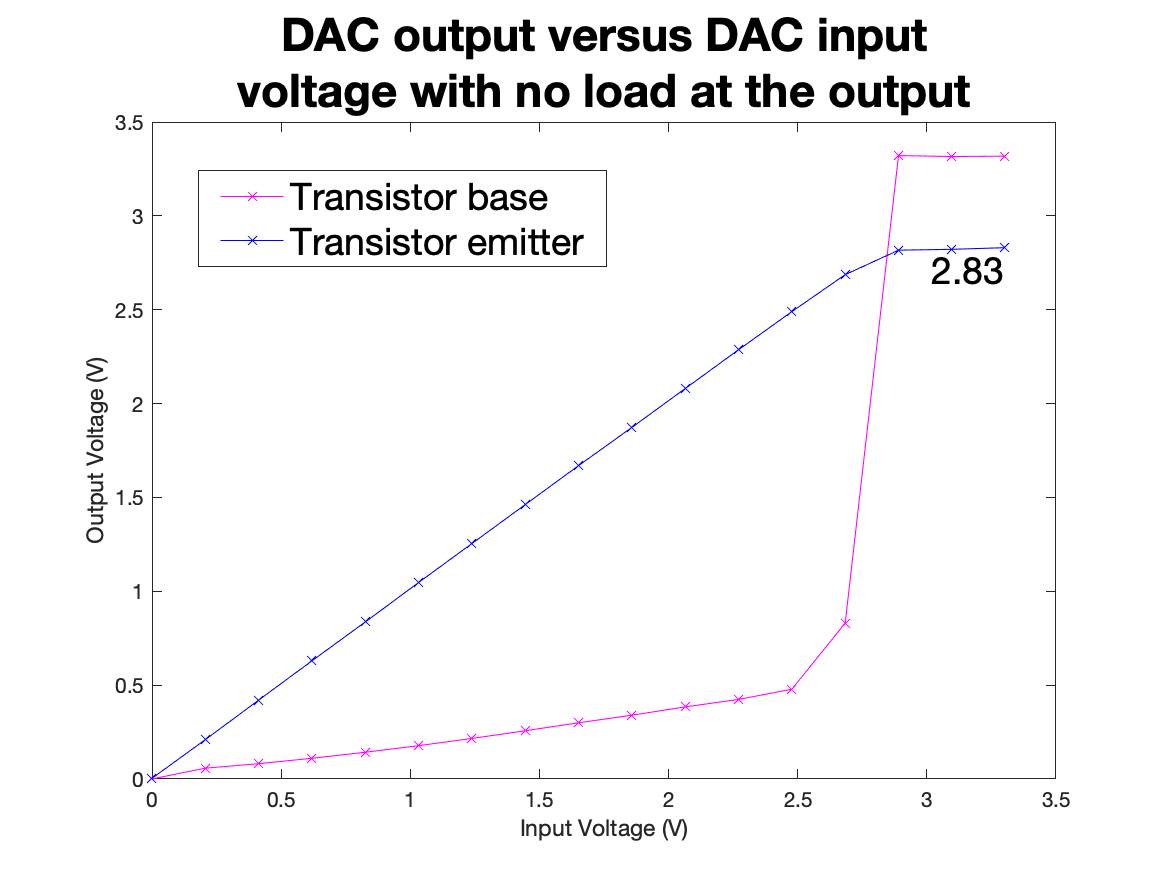
\includegraphics[width=\textwidth]{Figures/Testing/DAC_no_load}
        \caption{The input voltage versus the output voltage of the \gls{dac} with no load.}
        \label{fig:dac-voltage-range-no-load} %chktex 24
    \end{minipage}%
    \begin{minipage}{.5\textwidth}
        \centering
        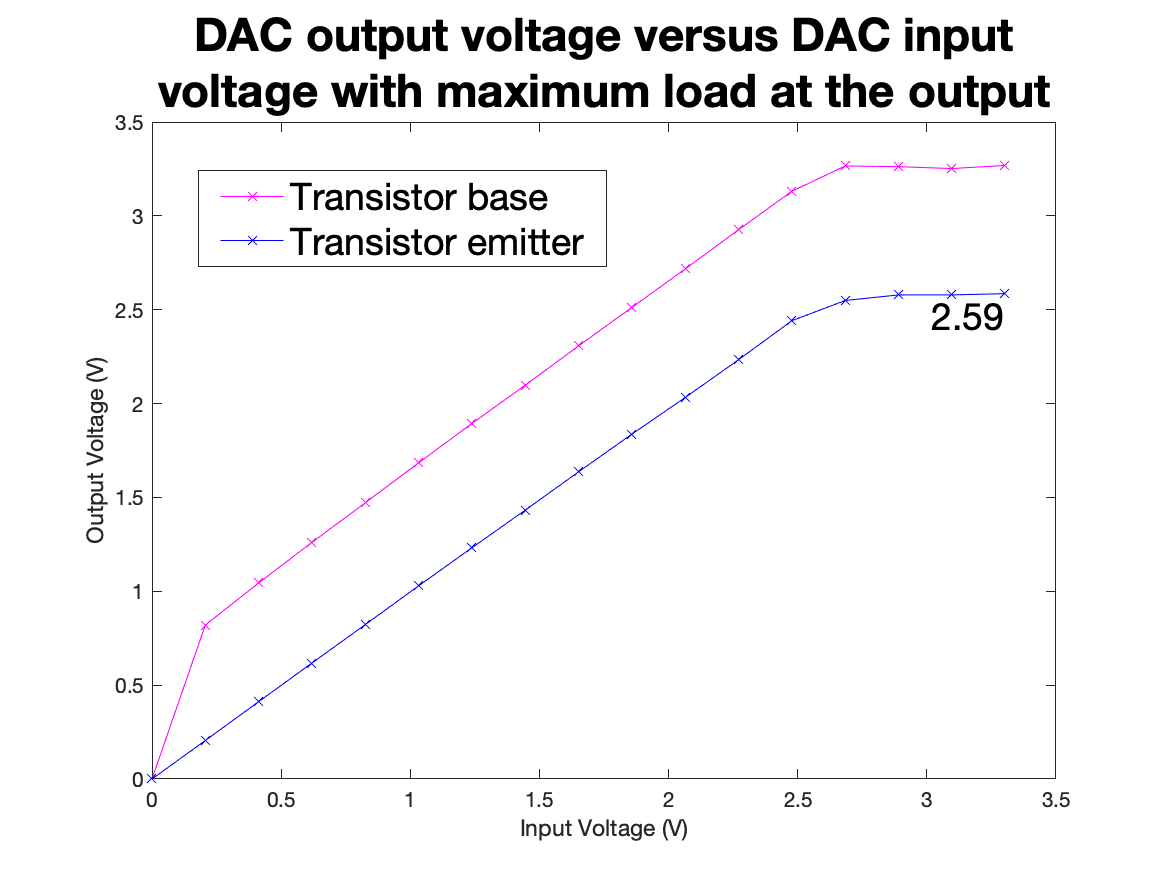
\includegraphics[width=\textwidth]{Figures/Testing/DAC_loaded}
        \caption{The input voltage versus the output voltage of the \gls{dac} with a load of $100\Omega$.}
        \label{fig:dac-voltage-range-loaded} %chktex 24
    \end{minipage}
\end{figure}

The results were graphed and are shown in~\reffig{fig:dac-voltage-range-no-load} and~\reffig{fig:dac-voltage-range-loaded}.
The voltage drop as a result $V_{BE}$ can clearly be seen on~\reffig{fig:dac-voltage-range-loaded}.
The unloaded output voltage was able to reach $2.83V$ and the loaded output voltage was able to reach $2.59V$ which are slightly higher than the predicted limits.

An alternate attempt was also made to achieve a higher voltage output by using the internal reference voltage of the \gls{dac}.
The internal reference voltage was set to $4 \times 1.21V = 4.84V$ and the \gls{dac} was instructed to output the maximum voltage.
As expected, this was not able to increase the output voltage; the base of the transistor still outputted $3.3V$ and the emitter still outputted $2.83V$ while unloaded.

Due to the voltage limitations, the \gls{dac} will have a limited output in future testing and implementation to prevent the output voltage not reaching the desired input voltage.
The output will be limited to $0V$ to $2.5V$ or $0$ to $775$ for fully loaded tests and the implementation and $0V$ to $2.7$ or $0$ to $837$ for unloaded tests.
When excluding the voltage readings above $2.5V$, the \gls{dac} was able to achieve a gain of $0.9837V/V$ and an offset $+0.0070V$ between the input voltage and output voltage when under maximum load. 

\textit{add LSB error = 0.00032V}

\section{ADC Accuracy}\label{sec:adc-accuracy}

The \gls{adc} will be tested by measuring a range of voltages produced by the \gls{dac} and comparing the voltage measured by a multimeter to the voltage measured by the \gls{adc}.
The \gls{adc} will be configured in 12-bit mode with each measurement taking 15 \gls{adc} clock cycles and 5 measurements will be taken and averaged to increase the accuracy of the measurement.
The accuracy of the \gls{adc} should ideally be $100\%$.

\begin{figure}[!h]
    \centering
    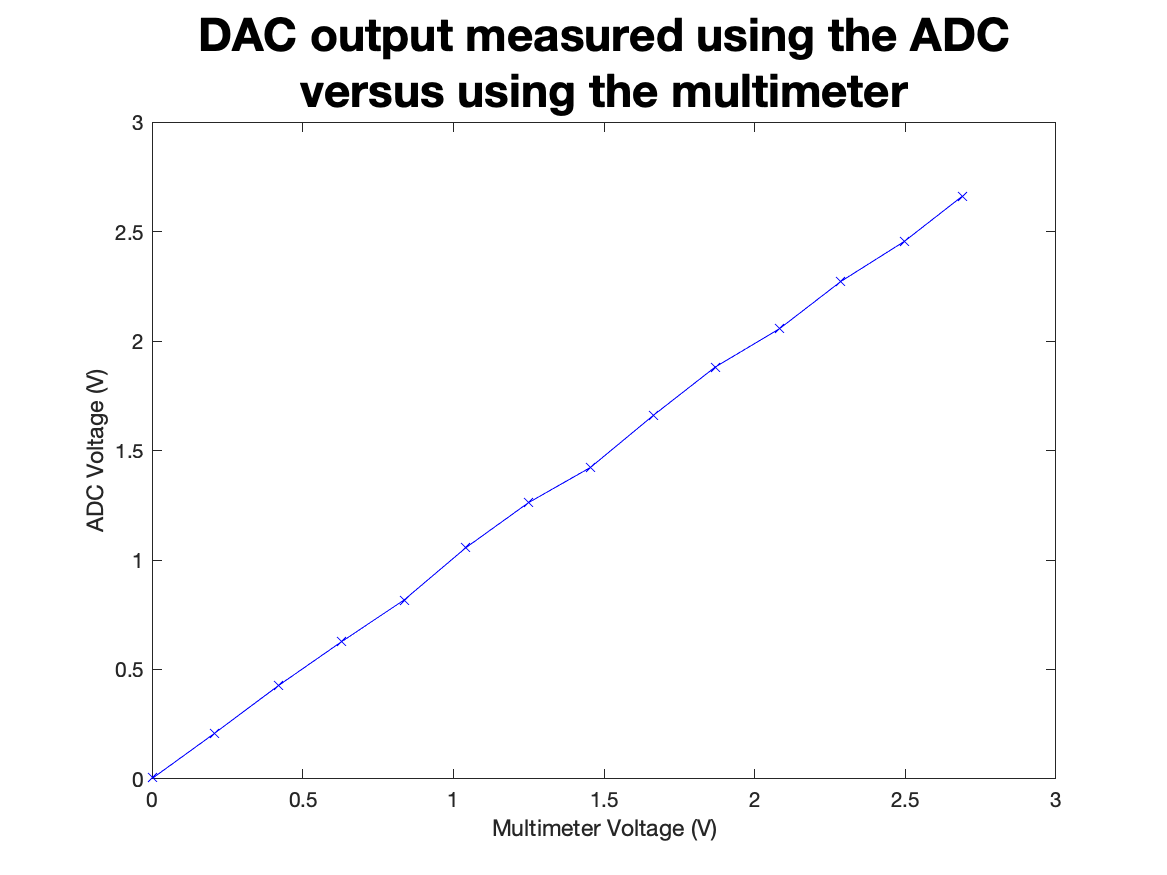
\includegraphics[width=0.5\textwidth]{Figures/Testing/ADC}
    \caption{The voltage output by the \gls{dac} measured by a multimeter versus measured by the \gls{adc}.}
    \label{fig:adc-accuracy} %chktex 24
\end{figure}

The results are shown in~\reffig{fig:adc-accuracy}. 
The \gls{adc} achieved a gain of $0.9877V/V$ and an offset of $0.0082V$ when compared to the multimeter.

\section{Calibration Resistance}\label{sec:calibration-resistance}

The calibration resistor will be measured by using the multimeter and by using the \gls{adc} with and without the gain applied.
The calibration resistance was specified to be $5\Omega \pm 0.25\%$, and thus it is expected to be between $4.9875$ and $5.0125\Omega$.

The calibration resistors were electrically disconnected, and the multimeter was used to measure the calibration resistor to be $5.25\Omega$ when the probes where applied directly across one of the parallel calibration resistor's terminals.
The multimeter cables measured $0.25\Omega$ when connected to each other and thus the final resistance of the calibration resistor was $5.00\Omega$.
It should be noted that the multimeter could only measure down to $0.01\Omega$ and thus the true resistance could range from $4.99\Omega$ to $5.01\Omega$.


\section{Resistance Measuring Accuracy}\label{sec:resistance-measuring-accuracy}

The method of measuring resistance involves getting a voltage reading of the calibration resistor and a sample resistor which is attached between the titanium electrode ports.
The resistance of the sample resistor is then calculated using the ratio between the voltage across the sample resistor and the calibration resistor.

This will be done using two methods: one with a single voltage from the \gls{dac} of $V_{DD}/2 = 1.65V$ and one with voltage sweep from the \gls{dac} with $50$ samples.
It was noticed during the testing phase that low voltage readings were not accurate as single bit errors caused large changes in the resistance reading and thus the range of voltages will be limited to $0.3V$ to $2.6V$ or $93$ to $806$ bits.
Both measurements will then be compared to the resistance measured by the multimeter.
The range of the resistors used will be $0\Omega$ to $10\Omega$ as this is the expected range for the gold electrodes.

\begin{figure}[!h]
    \centering
    \begin{minipage}{.5\textwidth}
        \centering
        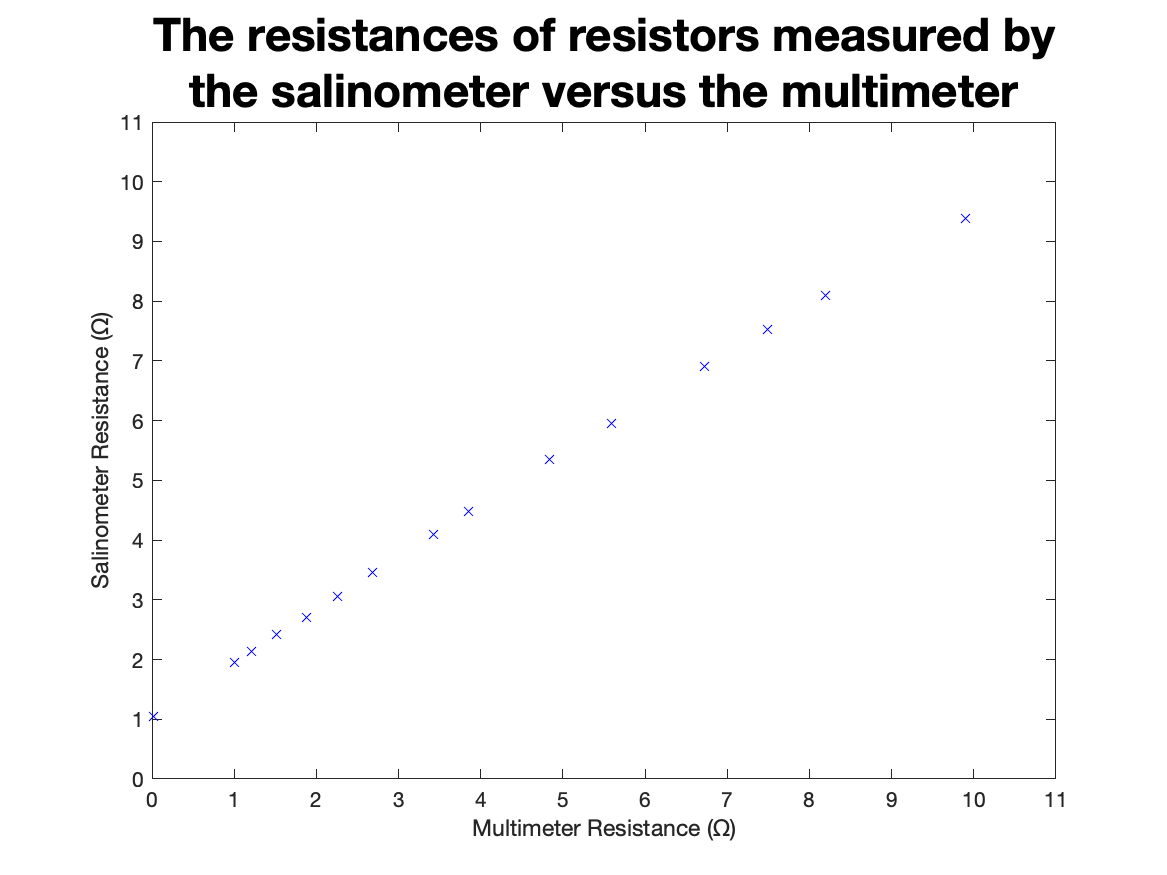
\includegraphics[width=\textwidth]{Figures/Testing/R_uncorrected}
        \caption{The resistance measuring test.}
        \label{fig:resistance-measuring-accuracy-uncorrected} %chktex 24
    \end{minipage}%
    \begin{minipage}{.5\textwidth}
        \centering
        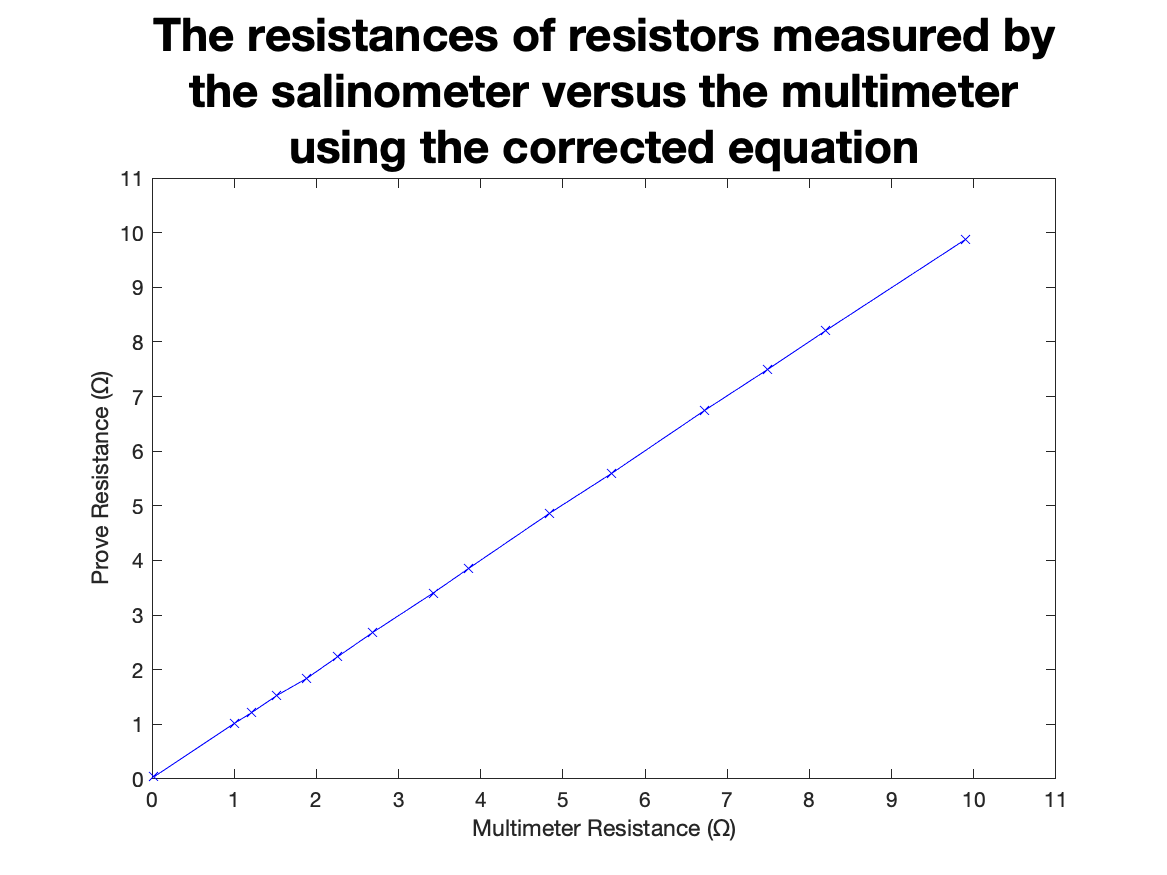
\includegraphics[width=\textwidth]{Figures/Testing/R_corrected}
        \caption{The resistance measuring test using the correction equation.}
        \label{fig:resistance-measuring-accuracy-corrected} %chktex 24
    \end{minipage}
\end{figure}

The results are shown in~\reffig{fig:resistance-measuring-accuracy-uncorrected}. 
The single voltage method and voltage sweep method were perfectly correlated with an $r^2$ value of $1.0000$, however there was a clear error between the actual resistance and the resistance measured by the salinometer.
This error was assumed to be due to the resistance of the switches and the traces.
While these values could be measured and corrected for, a more effective method would be to generate a curve of best fit and use this to correct the resistance readings.

The equation for how the measured resistance $R_{measured}$ was calculated is shown in \refeqn{eq:resistance-measuring}.
This equation is then expanded using the resistor divider formula, then simplified and all the constant values are combined into the constants $R_{\alpha}$, $R_{\beta}$, and $K$ as shown in \refeqn{eq:resistance-measuring-simplified}.
This equation is then rearranged to be a rational function using $p$ and $q$ coefficients as shown in \refeqn{eq:resistance-measuring-rational} which should give the equation of best fit for the data shown in \reffig{fig:resistance-measuring-accuracy-uncorrected}.

\begin{align}
    R_{measured} &= \lfrac{V_{resistor}}{V_{calibration}} \times R_{calibration} \label{eq:resistance-measuring} \\
    &= \lfrac{V_{DAC}{A_{gain}}\lfrac{R_{resistor} + r_{e1}}{R_{resistor} + R_1 + r_{e2}}}{V_{DAC}{A_{gain}}\lfrac{R_{calib} + r_{e3}}{R_{calib} + R_1 + r_{e4}}} \times R_{calibration} \nonumber \\
    &= \lfrac{R_{resistor} + r_{e1}}{R_{resistor} + R_1 + r_{e2}} \times \lfrac{R_{calibration}}{\left(\lfrac{R_{calib} + r_{e3}}{R_{calib} + R_1 + r_{e4}}\right)} \nonumber \\
    R_{measured} &= \lfrac{R_{resistor} + R_{\alpha}}{R_{resistor} + R_{\beta}} \times K \label{eq:resistance-measuring-simplified} \\
    &= \lfrac{KR_{resistor} + KR_{\alpha}}{R_{resistor} + R_{\beta}} \nonumber \\
    R_{measured} &= \lfrac{p_1 R_{resistor} + p_2}{R_{resistor} + q_2} \label{eq:resistance-measuring-rational}
\end{align}

The \refeqn{eq:resistance-measuring-rational} of best fit was confirmed using \texttt{MATLAB} giving $p_1 = 87.3433$, $p_2 = 92.3206$ and $q_1 = 0.0001$, $q_2 = 91.8310$ with an $r^2$ value of $1.0000$. 
\refeqn{eq:resistance-measuring-rational} could then be rearranged in terms of $R_{resistor}$ to give the correct resistance from the measured resistance $R_{measured}$ as shown in \refeqn{eq:resistance-measuring-corrected}.  
After applying this equation to the recorded data, the results were graphed and are shown in~\reffig{fig:resistance-measuring-accuracy-corrected} with an $r^2$ value of $1.0000$.

\begin{equation}\label{eq:resistance-measuring-corrected}
    R_{resistor} = \lfrac{p_2 - q_2 R_{measured}}{R_{measured} - p_1}
\end{equation}